\documentclass[simplex.tex]{subfiles}
% NO NEED TO INPUT PREAMBLES HERE
% packages are inherited; you can compile this on its own

\onlyinsubfile{
\title{NeuroData SIMPLEX Report: Subfile}
}

\begin{document}
\onlyinsubfile{
\maketitle
\thispagestyle{empty}

The following report documents the progress made by the labs of Randal~Burns and Joshua~T.~Vogelstein at Johns Hopkins University towards goals set by the DARPA SIMPLEX grant.

%%%% Table of Contents
\tableofcontents

%%%% Publications
\bibliographystyle{IEEEtran}
\begin{spacing}{0.5}
\section*{Publications, Presentations, and Talks}
%\vspace{-20pt}
\nocite{*}
{\footnotesize	\bibliography{simplex}}
\end{spacing}
%%%% End Publications
}

\subsection{Non-Parametric Shape Clustering}

We developed a prototype algorithm for 2-dimensional shape clustering, which
is invariant under affine transformations. This employs the procrustes
distance between two objects, which requires feature extraction to obtain
landmark points; see Fig.~\ref{fig:nonpar} for an example. 
We intend to apply a variant of this method to analyze neural synapses,
since we have such datasets from our collaborators. However, to this particular
dataset, the preprocessing techniques may be highly sophisticated, and a new
metric to compare different objects may be necessary. Moreover, these shapes are
3-dimensional. We are currently working on this project
with our collaborators, extending our existing  techniques to this 
particular dataset.

We also started working on a related, and more general, project.
We intend to develop non-parametric clustering algorithms with statistical
guarantees. We will use an energy-statistics based approach. Given
two datasets $X$ and $Y$, there is an energy function $\mathcal{E}(X,Y)$
test statistic which allows us to infer if $X$ and $Y$ have the same
distribution. Our results thus far suggest that this can be written
as a quadratic optimization problem
with quadratic constraints: 
\begin{equation}
\max_{x,z\in \mathbb{R}^N} x^T \Delta z \qquad \mbox{s.t. $x_i^2=1$, $x+z = 0$}
\end{equation}
where $\Delta$ is a dissimilarity data matrix.
There is not enough literature on
this interesting problem, so this will very likely lead to new methods which
can have interesting applications, in particular to neuroscience datasets.

\begin{figure}[h!]
\begin{cframed}
\centering
\begin{subfigure}[t]{0.45\textwidth}
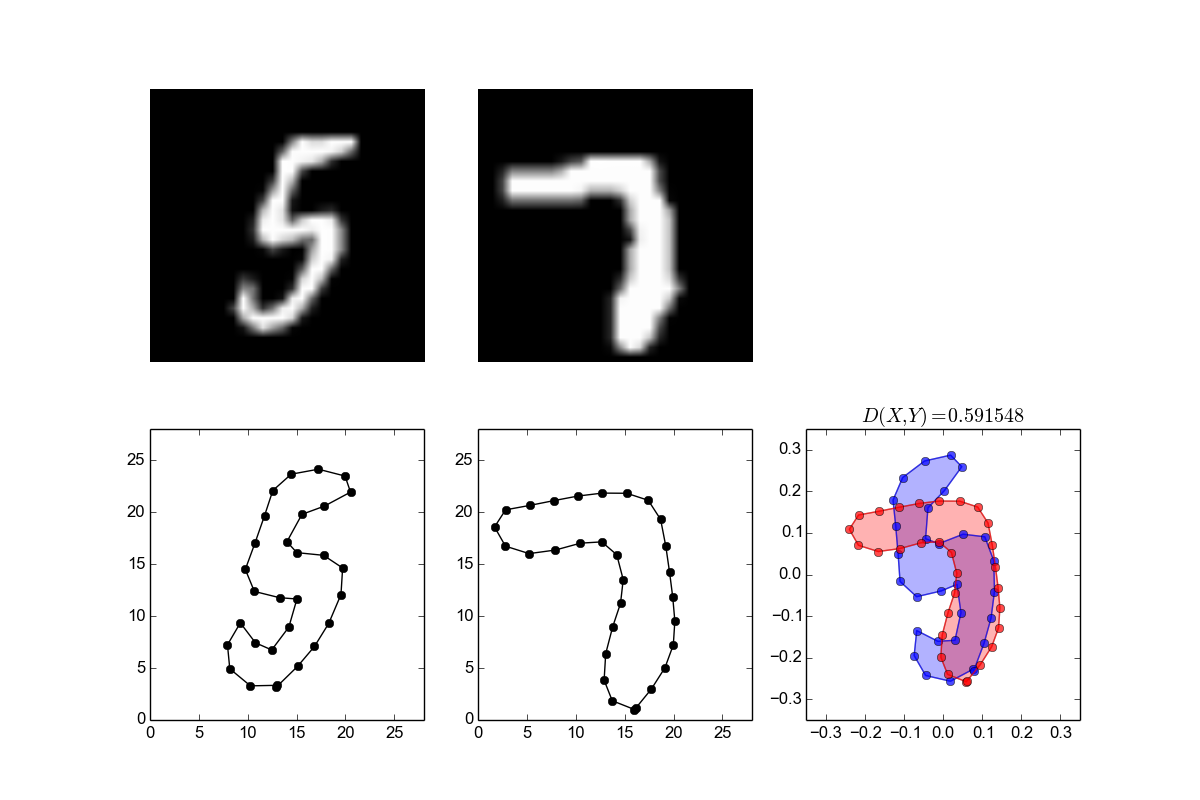
\includegraphics[width=\textwidth]{../../figs/nonpar57.png}
\label{fig:nonpar57}
\caption{
  MNIST digits with extracted landmarks and alignment.
  }
\end{subfigure}
\begin{subfigure}[t]{0.45\textwidth}
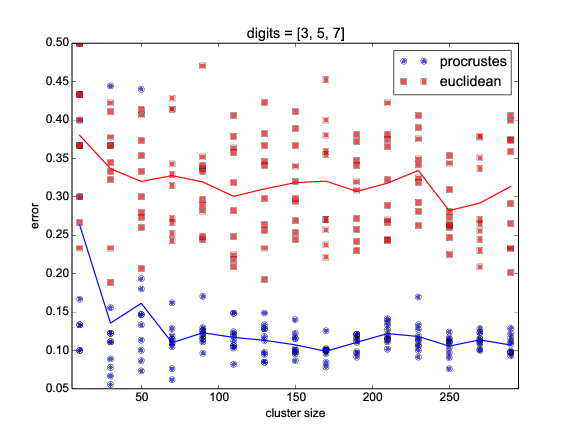
\includegraphics[width=\textwidth]{../../figs/nonPar357.png}
\label{fig:nonpar357}
\caption{
Classification error against the size of each
cluster (the three classes have the same number of points) is
shown in blue. The red line is standard
K-means with Euclidean distance for comparison.}
\end{subfigure}
\caption{
  MNIST handwritten digits and classification error results.
}
\label{fig:nonpar}
\end{cframed}
\end{figure}

\end{document}
